\documentclass[tikz]{standalone}
\begin{document}

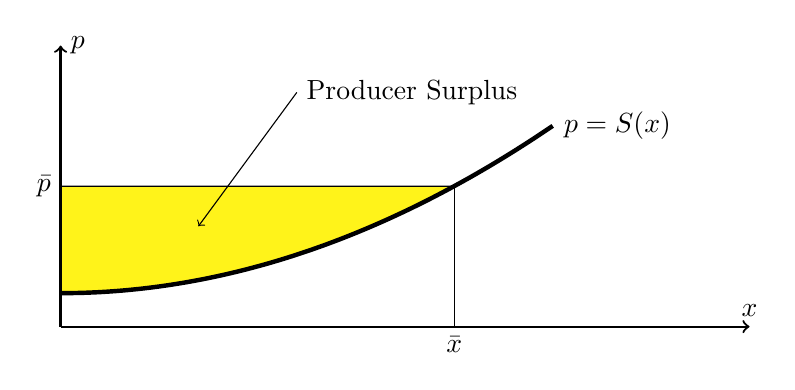
\begin{tikzpicture}[xscale=2.5,yscale=0.85]
  % shade region
  \draw[fill=yellow!90] plot[smooth, samples=100, domain=0:2] (\x,0.5+0.4*\x*\x) -| (0,0.5) ;

  % draw axes 
  \draw[thick,->] (0,0) -- (3.5,0) node[above] {$x$};
  \draw[thick,->] (0,0) -- (0,4.2) node[right] {$p$};

  % draw curves
  \draw[ultra thick,domain=0:2.5,smooth,variable=\x,black] plot ({\x},{0.5+0.4*\x*\x}) node[right] {$p=S(x)$};

  \draw (2,2.1) -- (2,0) node[below] {$\bar{x}$};
  \draw (2,2.1) -- (0,2.1) node[left] {$\bar{p}$};
  \draw[<-] (0.7,1.5)--(1.2,3.5) node[right] {Producer Surplus};

\end{tikzpicture}
\end{document} 
